\documentclass[a4paper]{article}
\usepackage{amsmath,amsfonts,amsthm,amssymb}
\usepackage{geometry}
\usepackage{graphicx}
\usepackage{physics}
\usepackage{booktabs}
\title{Vertex-Centre-Vertex Angle of Tetrahedra}
\author{Gordon Chan}

\begin{document}
\maketitle
\begin{center}
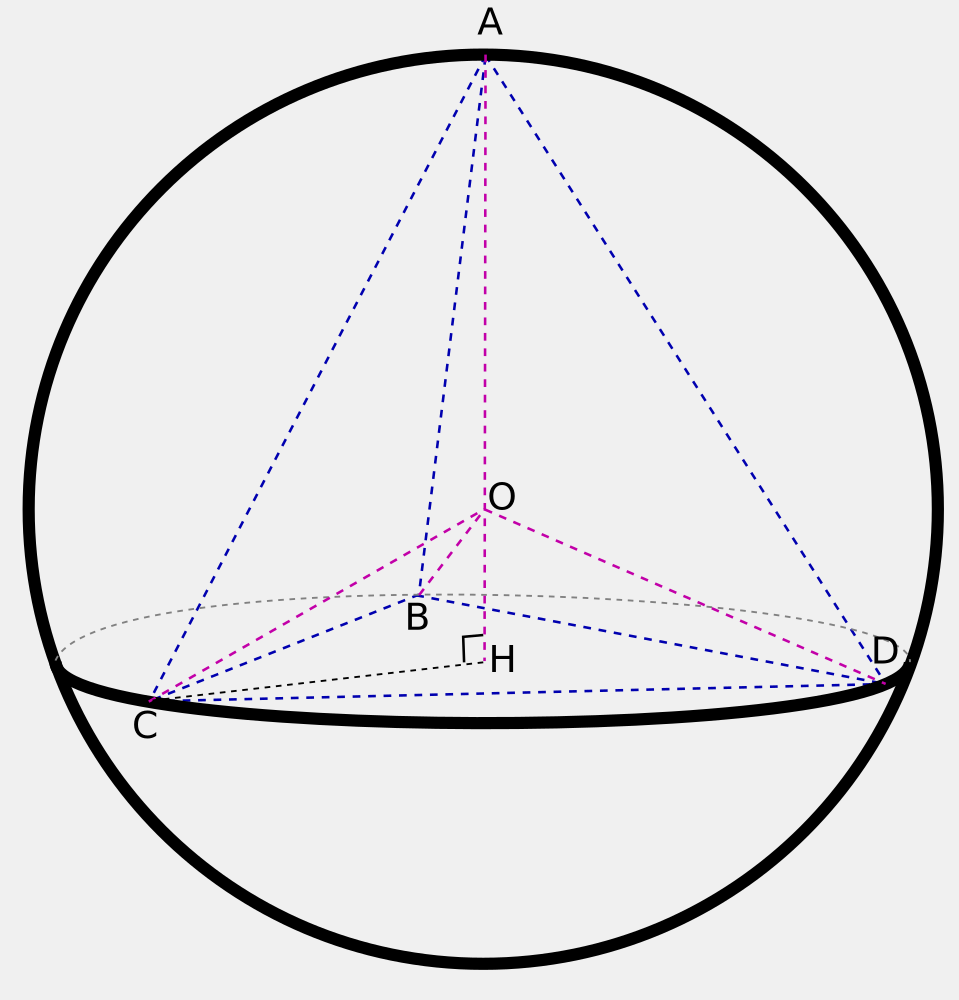
\includegraphics[width=0.9\textwidth]{tetrahedron.png}
\end{center}
\newpage

\section{Derivation of the Half Angle Formula}
The half angle formula is used to make the angle computed in the latter part
to be presented in a more simplified form.\\
By the unit circle identity and the double angle formula,
\[\begin{aligned}
    1&=\cos^2\frac\theta2-\sin^2\frac\theta2\\
    +\quad\bigg(\cos2\left(\frac\theta2\right)&=\cos^2\frac\theta2-\sin^2\frac\theta2\bigg)\\
    \midrule\\
    1+\cos\theta&=2\cos^2\frac\theta2\\
    \cos^2\frac\theta2&=\frac{1+\cos\theta}2\\
    \cos\frac\theta2&=\pm\sqrt{\frac{1+\cos\theta}2}
\end{aligned}\]

\newpage
\section{Computation of the Vertex-Centre-Vertex Angle of a Tetrahedron}
Let the side length of the tetrahedron be \(a\).\\
By similar triangles,
\[\begin{aligned}
    \frac hr&=\frac{\frac a2}a\\
    \frac hr&=\frac12\\
    h&=\frac r2
\end{aligned}\]
By the Pythagoras' theorem,
\[\begin{aligned}
	{(r+h)}^2+\left(\frac a2\right)^2&=a^2\\
    \left(r+\frac r2\right)^2&=a^2-\left(\frac a2\right)^2\\
    \left(\frac{3r}2\right)^2&=a^2-\frac{a^2}4\\
    \frac{9r^2}4&=\frac{3a^2}4\\
    r^2&=\frac{a^2}3\\
    r&=\frac a{\sqrt3}
\end{aligned}\]
By trigonometry,
\[\begin{aligned}
    \sin\varphi&=\frac ra\\
            &=\frac{\frac a{\sqrt3}}a\\
            &=\frac1{\sqrt3}
\end{aligned}\]
By angular sum of triangle,
\[\begin{aligned}
    \theta+\varphi+\varphi&=\pi\\
    \pi-\theta&=2\varphi\\
    \frac{(\pi-\theta)}2&=\varphi\\
    \sin\left(\frac\pi2-\frac\theta2\right)&=\sin\phi\\
    \cos\frac\theta2&=\frac1{\sqrt3}\\
    \cos^2\frac\theta2&=\frac13\\
    \frac{1+\cos\theta}2&=\frac13\\
    1+\cos\theta&=\frac23\\
    \cos\theta&=-\frac13\\
    \theta&=\boxed{\cos^{-1}\left(-\frac13\right)}\\
          &=1.9106332362\dots\\
          &=109.47122063\dots^\circ\\
          &\approx109.5^\circ
\end{aligned}\]

\section{Related: Structural Formula of a Methane Molecule}
Ew chemistry.
\begin{center}
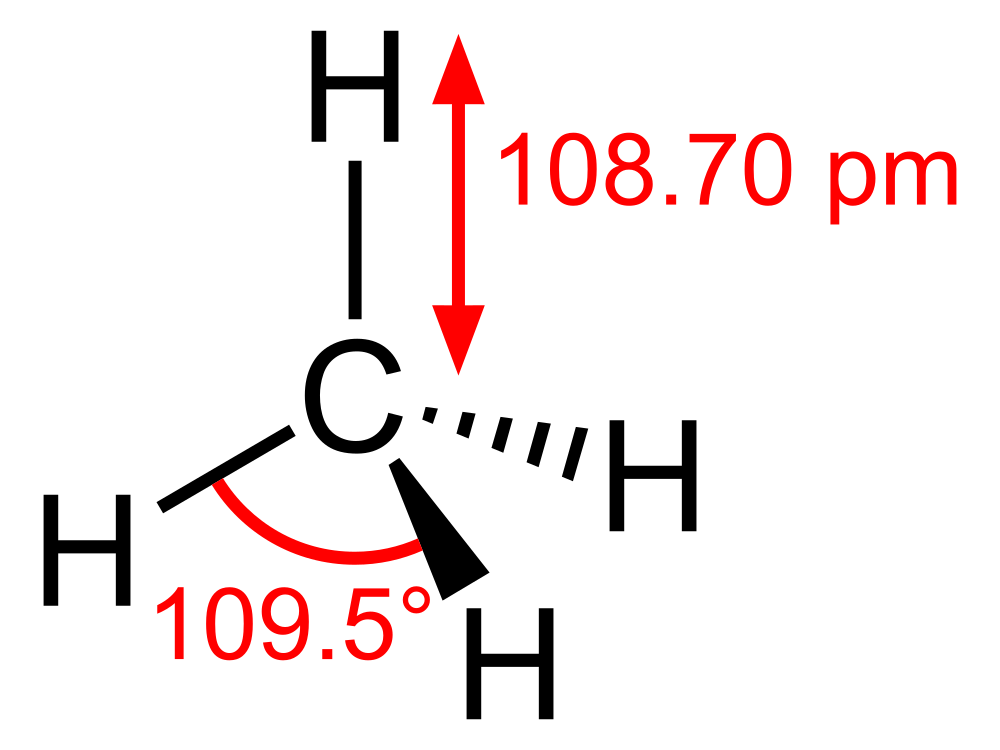
\includegraphics[width=0.69\textwidth]{methane.png}
\end{center}
\end{document}
